%!TEX root =  ../main.tex

\subsection{``Undo''}

\objective{Find and graph function inverses and their derivatives.}


We have seen that functions can be redefined as the composition of other, simpler
functions.  For example, $\frac{x^2+1}{2}$ can be seen as 1) squaring, 2) adding 1
, and 3) dividing by 2.  What if we wanted to ``undo'' the effects of this function?
We cannot simply do the opposite of each operation ($\frac{\sqrt{x} -1}{2}$ is not
the inverse) but must do the opposites \emph{backwards}.  This is called the
\textbf{inverse} of the function.  

\subsection{Swap $x$ and $y$}
In the example already mentioned, the inverse is $\pm\sqrt{2x-1}$.  What is wrong with 
this inverse?  It is not a function.  No even power has an inverse which is a function, because
there are infinitely many places where a particular output is reached from two different inputs.
Another way to think of inverses is reversing $x$ and $y$, making the output the input and
visa versa.  Only \textbf{one-to-one} functions --- where every $x$ has a \emph{unique}
$y$ --- will have inverses which are themselves functions.

Numerically, this shows how easy it is to construct an inverse of data: simply swap the
column labels for input and output!   This can be done algebraically too.  Staying with
the same example, we could follow the procedure of 1) swapping $x$ and $y$, and then
2) solving for $y$ to find the inverse of a function.

\begin{align*}
	y &= (x^2+1)/2 \\
	x &= (y^2+1)/2\\
	2x &= y^2+1\\
	2x - 1 &= y^2 \\
	\pm\sqrt{2x-1} &= y\\
\end{align*}

\subsection{S.I.F.T.}
But such examples fail when there are multiple places where $x$ appears in the equation
of $y$.  How can we find the inverse of $y=\sqrt{\frac{x-1}{2-x}}$  A helpful acronym to 
remember is such cases is S.I.F.T., which standard for
\begin{itemize}
\item[\textbf{S}pread] Clear the fractions, exponentiate the roots away, distribute the parentheses, etc.
\item[\textbf{I}solate] Move all the terms with the desired variable onto one side of the equation, and move all the other terms to the opposite side.
\item[\textbf{F}actor] Factor out the desired variable from all the terms on its side
\item[\textbf{T}ransfer] Divide off the term in parentheses, leaving the variable alone.
\end{itemize}
Returning to our hard example:

\begin{align*}
	y  &= \sqrt{\frac{x-1}{2-x}}\\
	x  &= \sqrt{\frac{y-1}{2-y}}\\
	x^2 &= \frac{y-1}{2-y}\\
	x^2(2-y) &= y-1 \\
	2x^2-x^2y &= y-1 &\text{finally spread out}\\
	2x^2 + 1 &= y + x^2y & \text{$y$ is isolated on the right}\\
	2x^2 + 1 &= y(1+x^2) & \text{factored out $y$}\\
	\frac{2x^2+1}{1+x^2} &= y & \text{transferred}
\end{align*}


\subsection{Graphically}
Inverses --- whether they are a function or not --- are a reflection across the line $y=x$.
This leads to some amazing properties of there derivatives.

Consider the function $f(x) = (x-1)^3+4$, a simple cubic function, shift right 1 and up 4.
It's derivative is easy to calculate: $f'(x)=3(x-1)^2$.  It's inverse somewhat more complicated,
but perhaps it is enough to sketch it, swapping $x$ and $y$ at every point, reflecting it over
the line $y=x$.

\begin{figure}[h]
\begin{centering}
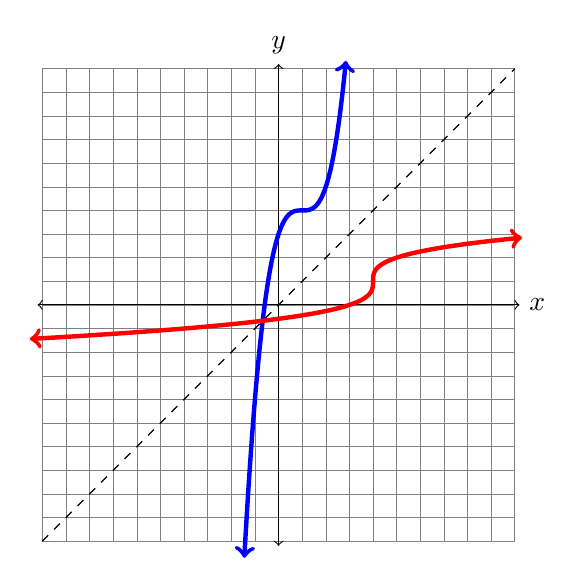
\begin{tikzpicture}[scale=0.3]
\draw[help lines] (-10,-10) grid (10,10);
\draw[<->] (-10.2,0) -- (10.2,0) node[anchor=west] {$x$};
\draw[<->] (0,-10.2) -- (0,10.2) node[anchor=south] {$y$};
\draw[dashed] (-10,-10) -- (10,10);
\draw[domain=-1.45:2.85,ultra thick,<->,samples=200,smooth,blue] plot (\x,{(\x-1)^3+4});
\draw[<->,domain=-1.44:2.85,samples=200,smooth,red,ultra thick]plot({(\x-1)*(\x-1)*(\x-1)+4},\x);
\end{tikzpicture}
\caption[Graphical example of inverses]{A function and its inverse, which are clearly reflections of each other across the line $y=x$.}
\end{centering}
\end{figure}

This can be done easily on the TI-8*.   First, enter the original function in $Y_1$ and graph
it.  Be sire you have a window appropriate to the function and it's inverse!  Next, select DRAW
and choose option 8: DrawInv, passing it the argument $Y_1$.  Press ENTER and 
you will be able to see the inverse.  Unfortunately, we cannot TRACE along it or any of the 
other tools we are used to for functions, but that hardly matters.  

Consider the tangent line through (2,5) on the original graph.  Hopefully, it is easy for
you to calculate that it follows the equation $y-5=3(x-2)$.  Enter this as $Y_2$.
Have the TI-8* draw its inverse.  This second line will pass through the point (5,2)
and have a reciprocal slope: $\frac{1}{3}$.

This shows that the derivative of the inverse is equal to the reciprocal of the derivate,
for every point $(x,y)$ which has been mapped onto $(y,x)$.
\index{derivative!of the inverse}
